\section{Experiments and Results}
\label{sec:results}

% Sources for every number in this section:
%   results/decisions.json                  -- automated selections (E2 vs E3, best loss, top-2)
%   runs/<run>/history.json                 -- per-epoch train loss / val mIoU (Fig. curves)
%   results/<run>/{val,test}/summary.json   -- mIoU, pixel acc, group mIoU
%   results/<run>/{val,test}/per_class_iou.csv, confusion.npy
% Test numbers only for the final configurations, evaluated once.

\textbf{Validation strategy and threats to validity.} All selection uses the
733-frame validation split, and every number in Table~\ref{tab:main} except
the test columns comes from it. Validation lacks four classes and is closer in
class composition to training than to test (total-variation distance 0.114
versus 0.246; Section~\ref{sec:data}), and test water and rock-bed come almost
entirely from the unseen \emph{creek} scene. Validation scores are therefore
likely to overstate test scores, so we report test IoU per class, not only
test mIoU, and treat the validation-to-test gap as a finding.

\textbf{Sanity check (E0).} U-Net/ResNet-18 memorized its 10 training images
to 98.0\% pixel accuracy (training loss 0.12) and 68.5\% mIoU after 200
epochs, passing the 95\% criterion. The residual mIoU gap is in classes covering
a few hundred pixels of the 10 images (\emph{pole}, \emph{log}, \emph{rock}),
which unweighted CE never predicts.

\subsection{Architecture and Encoder}
\label{sec:res_arch}

Deepening the U-Net encoder from ResNet-18 to ResNet-50 (E1$\to$E2) changed
validation mIoU by only $+0.6$ points (37.1$\to$37.7\%), smaller than the
1.0-point spread between two seeds of the same configuration
(Section~\ref{sec:res_pretrain}). Swapping the decoder for DeepLabV3+ at a
fixed ResNet-50 encoder (E2$\to$E3) gave $+5.6$ points (43.3\%), and the
automated rule selected DeepLabV3+. Most of that gap, however, is an artifact
of the metric on this split: both U-Nets sporadically predict \emph{sand} and
\emph{rock-bed}, which do not occur in validation, and so average in two
zero-IoU terms that DeepLabV3+ avoids. Over the 20 classes present in
validation the decoder gain shrinks to $+1.8$ points (41.5$\to$43.3\%; $+2.1$
averaged over the last five epochs), with
the largest per-class gains on \emph{vehicle} (54$\to$62\%) and
\emph{picnic-table} (45$\to$60\%), both objects whose extent benefits from
DeepLabV3+'s multi-scale context. The choice of DeepLabV3+ stands under both
definitions, but the effect is moderate, not large.

\begin{table*}[t]
  \centering
  \caption{Main results (\%). Val: best-epoch validation mIoU, the selection
  criterion, excluding \emph{void} and \emph{bridge}; GT-pres.: the same
  checkpoint scored only on the 20 classes present in validation
  (Section~\ref{sec:metrics}). Test columns are computed once, for every run
  whose weights survived (Section~\ref{sec:compute}); group: six-group
  traversability mIoU. The E7 test row uses its seed-1 replicate.}
  \label{tab:main}
  \footnotesize
  \begin{tabular}{@{}l l l l c c c c c c c c@{}}
    \toprule
     & & & & \multicolumn{2}{c}{Validation mIoU} & \multicolumn{3}{c}{Test} & \multicolumn{3}{c}{Rare-class IoU, test} \\
    \cmidrule(lr){5-6}\cmidrule(lr){7-9}\cmidrule(lr){10-12}
    ID & Arch. & Enc. & Loss & Val & GT-pres. & mIoU & pix.\ acc. & group & water & log & rock \\
    \midrule
    E1 & U-Net      & R18 & CE      & 37.1 & 40.8 & 34.2 & 76.0 & 58.6 & 1.0 & 43.8 & 2.2 \\
    E2 & U-Net      & R50 & CE      & 37.7 & 41.5 & 34.0 & 76.1 & 60.9 & 1.8 & 47.2 & 6.0 \\
    E3 & DeepLabV3+ & R50 & CE      & 43.3 & 43.3 & 37.0 & \textbf{77.4} & \textbf{62.7} & 4.6 & \textbf{48.1} & \textbf{14.9} \\
    E4 & DeepLabV3+ & R50 & wCE     & 33.7 & 37.1 & --   & --   & --   & --   & --   & --   \\
    E5 & DeepLabV3+ & R50 & Dice    & 42.3 & 44.5 & --   & --   & --   & --   & --   & --   \\
    E6 & DeepLabV3+ & R50 & Focal   & 41.1 & 43.2 & --   & --   & --   & --   & --   & --   \\
    E7 & DeepLabV3+ & R50 & CE+Dice & \textbf{44.2} & \textbf{46.5} & \textbf{37.7} & 76.5 & 60.0 & \textbf{6.4} & 48.0 & 9.9 \\
    E8 & DeepLabV3+ & R50 (scratch) & CE+Dice & 38.5 & 40.4 & 32.2 & 73.9 & 58.2 & 1.9 & 38.1 & 6.3 \\
    \midrule
    E9 & \multicolumn{3}{l}{E7, seed 1} & 45.2 & 47.5 & \multicolumn{6}{l}{(test results in the E7 row)} \\
    & \multicolumn{3}{l}{E7, seeds 0--1 (mean $\pm$ half-range)} & 44.7$\pm$0.5 & 47.0$\pm$0.5 & & & & & & \\
    \midrule
    \multicolumn{4}{@{}l}{RUGD baselines~\cite{wigness2019rugd}$^\dagger$} & 35.7--36.7 & & 31.8--32.2 & & & 1.8--5.3 & 40.2--43.1 & 8.9--13.3 \\
    \bottomrule
  \end{tabular}\\[2pt]
  \parbox{\textwidth}{\footnotesize $^\dagger$ResNet-50 PSPNet/UPerNet variants
  from Tables II, III, and V of~\cite{wigness2019rugd}: $688\times555$ input,
  80K iterations, mIoU averaged over the 24 RUGD classes as defined there, including \emph{bridge}. They are
  shown for context only and are not directly comparable.}
\end{table*}

\subsection{Loss Functions and Rare Classes}
\label{sec:res_loss}

On DeepLabV3+/ResNet-50, CE+Dice (E7) had the highest validation mIoU, 44.2\%
($+0.9$ over CE), and was selected; it also leads on GT-present mIoU (46.5\%
vs.\ 43.3\% for CE). The gain is concentrated in rare and mid-frequency
classes (Fig.~\ref{fig:perclass}): water 50$\to$54\%, log 30$\to$36\%,
container 6$\to$37\%, and concrete 2$\to$14\%, with frequent classes (tree,
grass, mulch, asphalt) unchanged to within one point and pixel accuracy
essentially flat (90.9$\to$90.6\%). Dice alone (E5) looks weaker under the
selection metric (42.3\%) only because its validation peak fell at epoch 7,
where it also predicts absent classes. Scored on GT-present classes its best
epoch reaches 46.9\%, tying CE+Dice (47.0\%), so the Dice term, not the CE
term, carries the rare-class gain. Focal loss (E6, 41.1\%) behaved like CE,
slightly better on rock (46\%) and log (34\%) but worse on pole, and was the
slowest per epoch. Median-frequency weighted CE (E4) was the clear failure:
33.7\% mIoU and $-5.0$ points of pixel accuracy (85.9\%). Its large weights on
rare classes made the model over-predict them, lowering IoU on the very
classes it targets (water 21\%, log 21\%, rock 25\%) as well as on frequent
ones (mulch 83$\to$74\%, tree 91$\to$86\%). It improved only a few
boundary-heavy classes such as fence (29$\to$35\%) and concrete (12\%).
\emph{Dirt}, \emph{sign}, and \emph{person} stayed at or near 0\% IoU on
validation under every loss.

\begin{figure}[t]
  \centering
  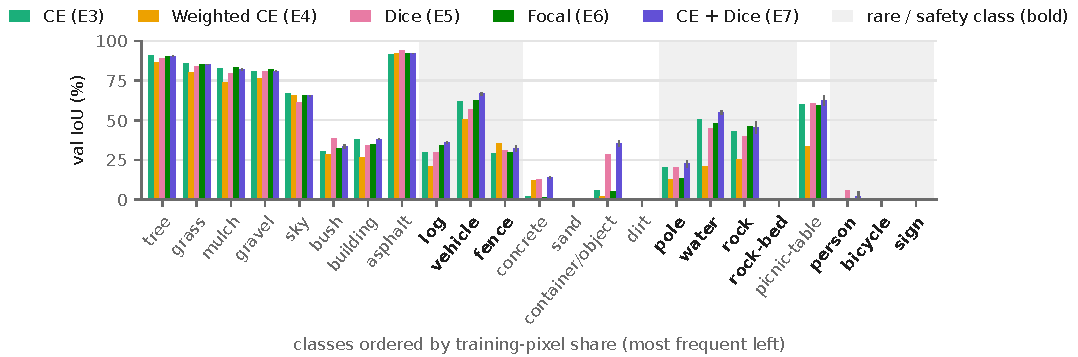
\includegraphics[width=\linewidth]{../results/figures/per_class_iou_losses.pdf}
  \caption{Per-class validation IoU by loss on DeepLabV3+/ResNet-50 (best
  epoch of each run), classes sorted by training frequency. Dice-based losses
  lift rare and mid-frequency classes without costing frequent ones; weighted
  CE lowers nearly every class.}
  \label{fig:perclass}
\end{figure}

\subsection{ImageNet Pretraining and Seed Variance}
\label{sec:res_pretrain}

Training the selected configuration from random initialization (E8) cost
5.7 points of validation mIoU (44.2$\to$38.5\%; 6.1 points GT-present). The
loss falls almost entirely on rare and mid-frequency objects (rock
43$\to$27\%, log 36$\to$25\%, container 37$\to$2\%, bush 32$\to$19\%, fence
33$\to$20\%), while frequent surfaces such as grass, asphalt, and gravel match
the pretrained model. E8 trails E7 at every epoch, by about 10 points early
and about 5 late, and ends at a higher training loss (0.43 vs.\ 0.33). The
gap was still narrowing, so this measures the benefit of pretraining under a
25-epoch budget, not at convergence.

\textbf{How noisy are these comparisons?} Two sources of noise matter. First,
validation mIoU fluctuates by 1--2 points from epoch to epoch after about
epoch 15 (Fig.~\ref{fig:curves}), and picking the best of 25 epochs rewards
single-epoch spikes. E3's 43.3\%, E7's 44.2\%, and E8's 38.5\% all sit one to
two points above the level each run settles at. Second, only one seed rerun
finished (Section~\ref{sec:compute}). The two seeds of CE+Dice differ by
1.0 point at their best epochs and by 2.3 points averaged over their last
five epochs (42.4 vs.\ 44.7\%), but by only 0.8 points on GT-present mIoU
(46.6 vs.\ 47.4\%). Much of the noise in the headline metric thus comes from
sporadic predictions of classes absent from validation. On the steadier
measure (GT-present, last-five-epoch mean) the ranking is: Dice (46.7) $\approx$
CE+Dice (46.6, 47.4) $>$ CE (43.5) $\approx$ focal (43.1) $>$ U-Net/R50 (41.4)
$\approx$ U-Net/R18 (40.6) $\approx$ no pretraining (40.5) $>$ weighted CE
(36.6). The Dice-based losses' gain over CE (about 3 points), the
pretraining gain (about 6), and weighted CE's loss (about 7) clearly exceed seed
noise. The encoder effect (0.8), CE+Dice versus Dice, and focal versus CE do
not. The decoder effect (2.1) is likely real but not by a wide margin. With
two seeds of one configuration these are rough bounds, not confidence
intervals.

\begin{figure}[t]
  \centering
  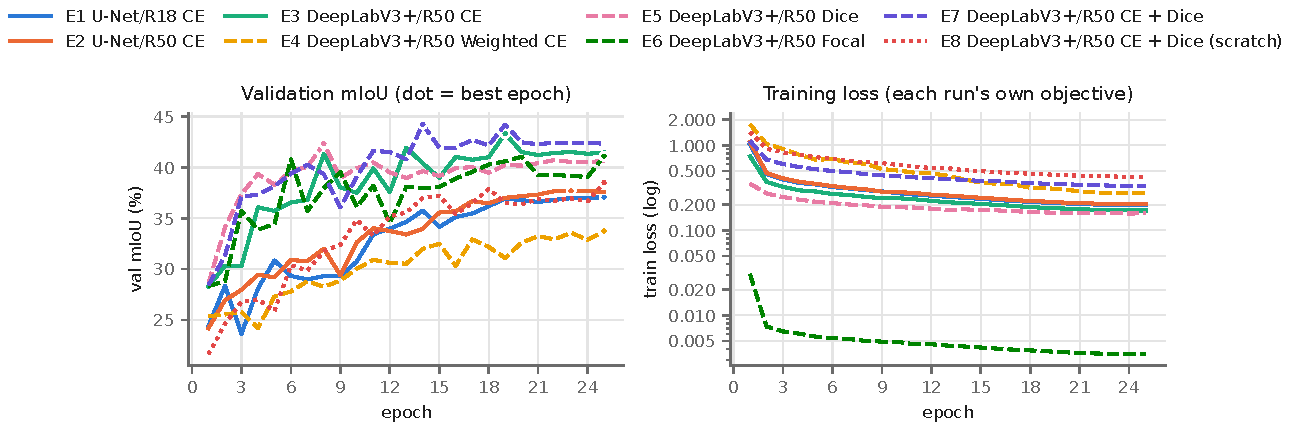
\includegraphics[width=\linewidth]{../results/figures/training_curves.pdf}
  \caption{Training loss and validation mIoU per epoch. After about epoch 15
  validation mIoU fluctuates by 1--2 points, so best-epoch selection favors
  single-epoch spikes. The run without pretraining (E8) trails its pretrained
  counterpart at every epoch, by about 10 points early and 5 points late.}
  \label{fig:curves}
\end{figure}

\subsection{Test Results and the Validation-to-Test Gap}
\label{sec:res_test}

On test, the selected CE+Dice model reaches 37.7\% mIoU, against 37.0\% for
CE (E3), 34.0--34.2\% for the U-Nets, and 32.2\% without pretraining
(Table~\ref{tab:main}). The ordering of architectures and of pretraining
matches validation, but CE+Dice's lead over CE shrinks to 0.7 points, within
seed noise, and CE is ahead on pixel accuracy, group mIoU, and rock. All
models lose 3--8 points of mIoU and 14--16 points of pixel accuracy from
validation to test (90--91\% to 74--77\%). The loss is almost entirely the
\emph{creek} sequence: it is 43\% of test pixels but produces 79--81\% of
every model's test errors, and it contains all of the test split's water and
rock-bed. Without creek, test mIoU is 49.3\% for CE+Dice, 47.9\% for CE,
43.5--44.3\% for the U-Nets and E8, and pixel accuracy is 90--92\%, on par
with validation. The validation-to-test gap is thus one unseen scene, not a
uniform drop, and is analyzed in Section~\ref{sec:error}. Our test mIoU is
above the RUGD baselines (31.8--32.2\%), though protocols differ
(Table~\ref{tab:main} footnote).

\subsection{Traversability Groups}
\label{sec:res_groups}

Mapping to six groups raises test mIoU from 37.7\% to 60.0\% for CE+Dice
(62.7\% for CE). Group IoU is high for obstacle (84\%), sky (82\%), and
vegetation (77\%), moderate for smooth (54\%) and rough ground (57\%), and
near zero for water (6\%). Coarsening helps most where fine-class errors stay
within a group, such as gravel versus rock-bed or grass versus bush, but
cannot help water, whose errors cross into the ground groups
(Section~\ref{sec:error}). CE's higher group mIoU comes mainly from rough
ground (67\% vs.\ 57\%), where CE+Dice labels more of creek's rock-bed as
smooth-ground mulch.

\subsection{Cross-Dataset Test on RELLIS-3D (Stretch Goal)}
\label{sec:res_rellis}

Zero-shot on the 1,672-frame RELLIS-3D test split, CE+Dice reaches 43.4\%
group mIoU with \emph{mud} ignored (43.6\% with mud scored as rough ground;
CE: 42.9\%), a drop of 16.6 points from its 60.0\% on RUGD test. The drop is
uneven. Sky (95\%) and vegetation (85\%) transfer, and even improve, since
they dominate RELLIS-3D frames (84\% of labeled pixels). Obstacles fall to
53\%, smooth ground to 25\%, and rough ground (\emph{rubble}, under 0.1\% of
pixels) and water (2\%) essentially fail. RELLIS-3D's dirt and asphalt are
predicted as vegetation or obstacle as often as ground (37\% recall), and its
puddles mostly as vegetation (49\%). The model's notion of ``ground'' is tied
to RUGD's mulch-and-gravel trails, and the safety-relevant groups are the
ones that transfer worst.
